\chapter{जननीय विकास और पुष्पन का नियंत्रण}\label{ch:b2:plant-flowering}

गुलदाउदी उगाने वाला बत्तियाँ बदलकर किसी हरितगृह को क्रिसमस या ईस्टर पर
फुला सकता है; वसंत में बोया गया कोई शीत-गेहूँ कभी फूलता ही नहीं, क्योंकि
उसने ठंड नहीं देखी; और जिस कॉकलबर ने अपनी क्रांतिक लंबाई से लंबी एक भी
रात देख ली हो वह फूलने को प्रतिबद्ध हो जाता है, आगे चाहे कुछ भी हो। किसी
पौधे के पास कोई पंचांग नहीं है, पर उसके पास घड़ियाँ, तापमापी और प्रकाश-मापी
हैं, और वह उन्हीं की गवाही पर वर्ष में एक बार निर्णय लेता है कि जो
\omterm{def:b2:plant-meristems:meristem}{विभज्योतक} अब तक पत्तियाँ बना रहा था उसे ऐसे \omterm{def:b2:plant-meristems:meristem}{विभज्योतक} में बदल दे जो कोई
\omterm{def:b2:angiosperm-reproduction:flower}{पुष्प} बनाएगा। यह अध्याय उस निर्णय का उस पत्ती से, जो रात नापती है, उस
\omterm{def:b2:plant-meristems:meristem}{विभज्योतक} तक पीछा करता है जो अपना कार्यक्रम बदलता है, फिर जीनों के किसी
कूट से \omterm{def:b2:angiosperm-reproduction:flower}{पुष्प} का बनना, और चक्र के दूसरे सिरे पर वह उलटा संक्रमण: यानी वह
\omterm{def:b2:angiosperm-reproduction:seed}{बीज} जो तब तक अंकुरित नहीं होगा जब तक उसे न बताया जाए कि ऋतु ठीक है।

\section{पुष्पन तक का संक्रमण}

\begin{definition}[पुष्पीय संक्रमण और प्रेरण]\label{def:b2:plant-flowering:transition}
\index{पुष्पीय संक्रमण}\index{पुष्पीय प्रेरण}\index{पुष्पक्रम विभज्योतक}
कोई कायिक \omterm{def:b2:plant-meristems:meristem}{प्ररोह शीर्षस्थ विभज्योतक} अनिश्चित काल तक ऐसी पत्तियाँ बनाता
है जिनके हर कक्ष में एक कलिका होती है। \emph{पुष्पीय संक्रमण} पर वह
\emph{पुष्पक्रम \omterm{def:b2:plant-meristems:meristem}{विभज्योतक}} बन जाता है, जो सहपत्र बनाता है और, उनके
कक्षों में, \emph{पुष्पीय \omterm{def:b2:plant-meristems:meristem}{विभज्योतक}}, जिनमें से हर एक निश्चित है: वह
बाह्यदल, दलपत्र, \omterm{def:b2:angiosperm-reproduction:flower}{पुंकेसर} और \omterm{def:b2:angiosperm-reproduction:flower}{अंडप} बनाकर रुक जाता है। यह परिवर्तन
\emph{पुष्पीय प्रेरण} से चलता है --- यानी कोई ऐसा संकेत जो पत्तियों से
आता है या पौधे की अपनी शरीरक्रिया में उठता है और
\omterm{def:b2:plant-meristems:meristem}{विभज्योतक} के पहचान-जीन बदल देता है। एकवर्षी एक बार फूलकर मर जाते हैं;
बहुवर्षी हर वर्ष कुछ \omterm{def:b2:plant-meristems:meristem}{विभज्योतकों} से फूलते हैं और बाक़ी को कायिक रखते
हैं। वह समय तय करता है कि \omterm{def:b2:plant-life-cycles:heterospory}{पराग} \omterm{def:b2:plant-life-cycles:heterospory}{पराग} से मिलेगा या नहीं, कि
\omterm{def:b2:angiosperm-reproduction:seed}{बीज} पाले से पहले पकेंगे या नहीं, और कि \omterm{def:b2:angiosperm-reproduction:flower}{पुष्प} तभी खुलेगा या नहीं जब उसका
परागक उड़ता हो: यह प्रबल वरण के अधीन है, और पौधों ने ऋतु पढ़ने के कई
रास्ते विकसित किए हैं।
\end{definition}

\begin{proposition}[दीप्तिकालिता: पौधा रात नापता है]\label{prop:b2:plant-flowering:photoperiod}
\index{दीप्तिकालिता}\index{अल्पदिवसी पौधा}\index{दीर्घदिवसी पौधा}\index{फ़ाइटोक्रोम}
अनेक पौधे दिन की लंबाई के उत्तर में फूलते हैं। \emph{अल्पदिवसी
पौधे} (गुलदाउदी, सोयाबीन, धान, कॉकलबर) तब फूलते हैं जब
दिन किसी क्रांतिक लंबाई से छोटा हो --- यानी शरद में या वसंत में;
\emph{दीर्घदिवसी पौधे} (पालक, गेहूँ, तिपतिया, \emph{Arabidopsis})
तब जब वह लंबा हो --- यानी आरंभिक ग्रीष्म में; और \emph{दिन-उदासीन} पौधे
(टमाटर, मक्का) तब फूलते हैं जब वे पर्याप्त बड़े हो जाएँ। पौधा जो नापता है
वह वास्तव में अटूट \emph{रात} की लंबाई है: कोई
\omterm{prop:b2:plant-flowering:photoperiod}{अल्पदिवसी पौधा} दीर्घरात्रि पौधा है, और किसी लंबी रात के
बीचोंबीच प्रकाश की एक झलक उसका प्रभाव रद्द कर देती है, जबकि किसी लंबे दिन
में अंधकार की कोई अवधि नहीं करती। वह मापन \emph{पत्तियों} में होता है,
रंजक \emph{फ़ाइटोक्रोम} द्वारा --- यानी ऐसा प्रोटीन जो पकड़े गए हर फ़ोटॉन
के साथ लाल-अवशोषी रूप और दूर-लाल-अवशोषी रूप के बीच पलटता है, इसलिए उसकी
अवस्था प्रकाश दर्ज कर लेती है --- और उसे लगभग चौबीस घंटे की किसी आंतरिक
\emph{सर्केडियन घड़ी} के विरुद्ध पढ़ा जाता है: पुष्पन तब चलता है जब प्रकाश
उस घड़ी की किसी विशेष कला से मेल खाए, और यह केवल सही
दिन-लंबाई पर ही होता है।
\end{proposition}
\begin{proof}[प्रमाण-सामग्री]
गार्नर और ऐलार्ड (1920) ने पाया कि तंबाकू का कोई उत्परिवर्ती केवल
किसी शीतकालीन हरितगृह के छोटे दिनों में फूलता था, और कि गर्मी भर
अंतराल पर बोए गए सोयाबीन सब सितंबर में एक साथ फूले: यानी दिन की लंबाई ने,
न कि आयु या ताप ने, वह तारीख़ तय की। हैमनर और बॉनर
(1938) ने कॉकलबर से दिखाया कि एक ही लंबी रात पर्याप्त थी, कि
रात के बीचोंबीच मिनट भर का प्रकाश उस प्रभाव को मिटा देता था,
और कि रात बदले बिना दिन छोटा करने से कोई प्रेरण नहीं होता। बोर्थविक और
हेंड्रिक्स (1952) ने पाया कि सबसे असरदार प्रकाश लाल था और कि लाल के
तुरंत बाद दिया गया दूर-लाल प्रकाश उसे रद्द कर देता था --- यानी फ़ाइटोक्रोम
का हस्ताक्षर, जो 1959 में अलग किया गया। किसी अप्रेरित पौधे पर किसी एक
प्रेरित पत्ती को ग्राफ़्ट करने से पूरा पौधा फूल गया: यानी वह पत्ती कोई संकेत भेजती है।
\end{proof}

\begin{omfigure}
\begin{tikzpicture}[every node/.style={font=\scriptsize}]
  \foreach \y/\lab/\res in {3.6/{लंबा दिन, छोटी रात}/{पुष्प नहीं}, 2.7/{छोटा दिन, लंबी रात}/{फूलता है}, 1.8/{लंबी रात, प्रकाश की एक झलक से टूटी}/{पुष्प नहीं}, 0.9/{लंबा दिन, अंधकार से टूटा}/{पुष्प नहीं}} {
    \node[anchor=east, align=right] at (-0.2,\y) {\lab};
    \node[anchor=west, omThm] at (8.6,\y) {\res};
  }
  % bars: 24 h = 8 cm; light yellow, dark grey
  \fill[omExo!30] (0,3.4) rectangle (8,3.8); \fill[yellow!50!orange!40] (0,3.4) rectangle (5.4,3.8);
  \fill[omExo!30] (0,2.5) rectangle (8,2.9); \fill[yellow!50!orange!40] (0,2.5) rectangle (3.0,2.9);
  \fill[omExo!30] (0,1.6) rectangle (8,2.0); \fill[yellow!50!orange!40] (0,1.6) rectangle (3.0,2.0); \fill[yellow!50!orange!40] (5.4,1.6) rectangle (5.55,2.0);
  \fill[omExo!30] (0,0.7) rectangle (8,1.1); \fill[yellow!50!orange!40] (0,0.7) rectangle (5.4,1.1); \fill[omExo!30] (2.6,0.7) rectangle (2.9,1.1);
  \draw[thick, ->] (0,0.3) -- (8.2,0.3); \foreach \x/\l in {0/0,2/6,4/12,6/18,8/24} \draw (\x,0.35) -- (\x,0.25) node[below] {\l};
  \node[below] at (4,-0.05) {घंटे};
  \draw[dashed, omDef] (5.4,0.3) -- (5.4,4.0); \node[omDef, above] at (5.4,4.0) {क्रांतिक रात्रि-लंबाई};
\end{tikzpicture}

{\small हैमनर और बॉनर का कॉकलबर, यानी कोई \omterm{prop:b2:plant-flowering:photoperiod}{अल्पदिवसी पौधा}। वह
क्रांतिक लंबाई से लंबी किसी रात के बाद फूलता है; रात के बीचोंबीच मिनट भर
का प्रकाश उस प्रेरण को रद्द कर देता है, जबकि दिन में अंधकार की कोई अवधि
नहीं करती। वह पौधा रात नापता है।}
\end{omfigure}

\begin{definition}[फ़्लोरिजन]\label{def:b2:plant-flowering:florigen}
\index{फ़्लोरिजन}\index{FLOWERING LOCUS T}
पत्ती जो संकेत भेजती है उसे 1937 में \emph{फ़्लोरिजन} नाम मिला और
सत्तर वर्ष बाद उसकी पहचान एक छोटे प्रोटीन के रूप में हुई, यानी
जीन \emph{FLOWERING LOCUS T} (FT) के उत्पाद के रूप में। पत्ती में वह घड़ी
और फ़ाइटोक्रोम मिलकर FT को केवल तभी चालू करते हैं जब दिन की लंबाई ठीक हो
(\emph{Arabidopsis} में, जो \omterm{prop:b2:plant-flowering:photoperiod}{दीर्घदिवसी पौधा} है, तब जब प्रकाश
घड़ी-नियंत्रित सक्रियक CONSTANS के दोपहर-बाद के शिखर से मेल खाए);
वह FT प्रोटीन फ्लोएम में घुसता है, शर्करा-धारा के साथ प्ररोह-शीर्ष तक
जाता है, और वहाँ, किसी साथी प्रोटीन के साथ, वे जीन चालू करता है जो
\omterm{def:b2:plant-meristems:meristem}{विभज्योतक} को बदल देते हैं। वही प्रोटीन धान का भी फ़्लोरिजन है, जो
\omterm{prop:b2:plant-flowering:photoperiod}{अल्पदिवसी पौधा} है, और जिसमें वह घड़ी उसे उलटी दिशा में जोड़ती है।
ग्राफ़्ट-प्रयोग, फ्लोएम में उस प्रोटीन का अभिगमन, और उन पौधों का पुष्पन
जिनमें FT किसी पत्ती-विशिष्ट उन्नायक से अभिव्यक्त होता है --- सब एक ही
बात कहते हैं: \omterm{def:b2:angiosperm-reproduction:flower}{पुष्प} का निर्णय पत्ती में होता है और कार्यान्वयन कलिका में।
\end{definition}

\begin{omfigure}
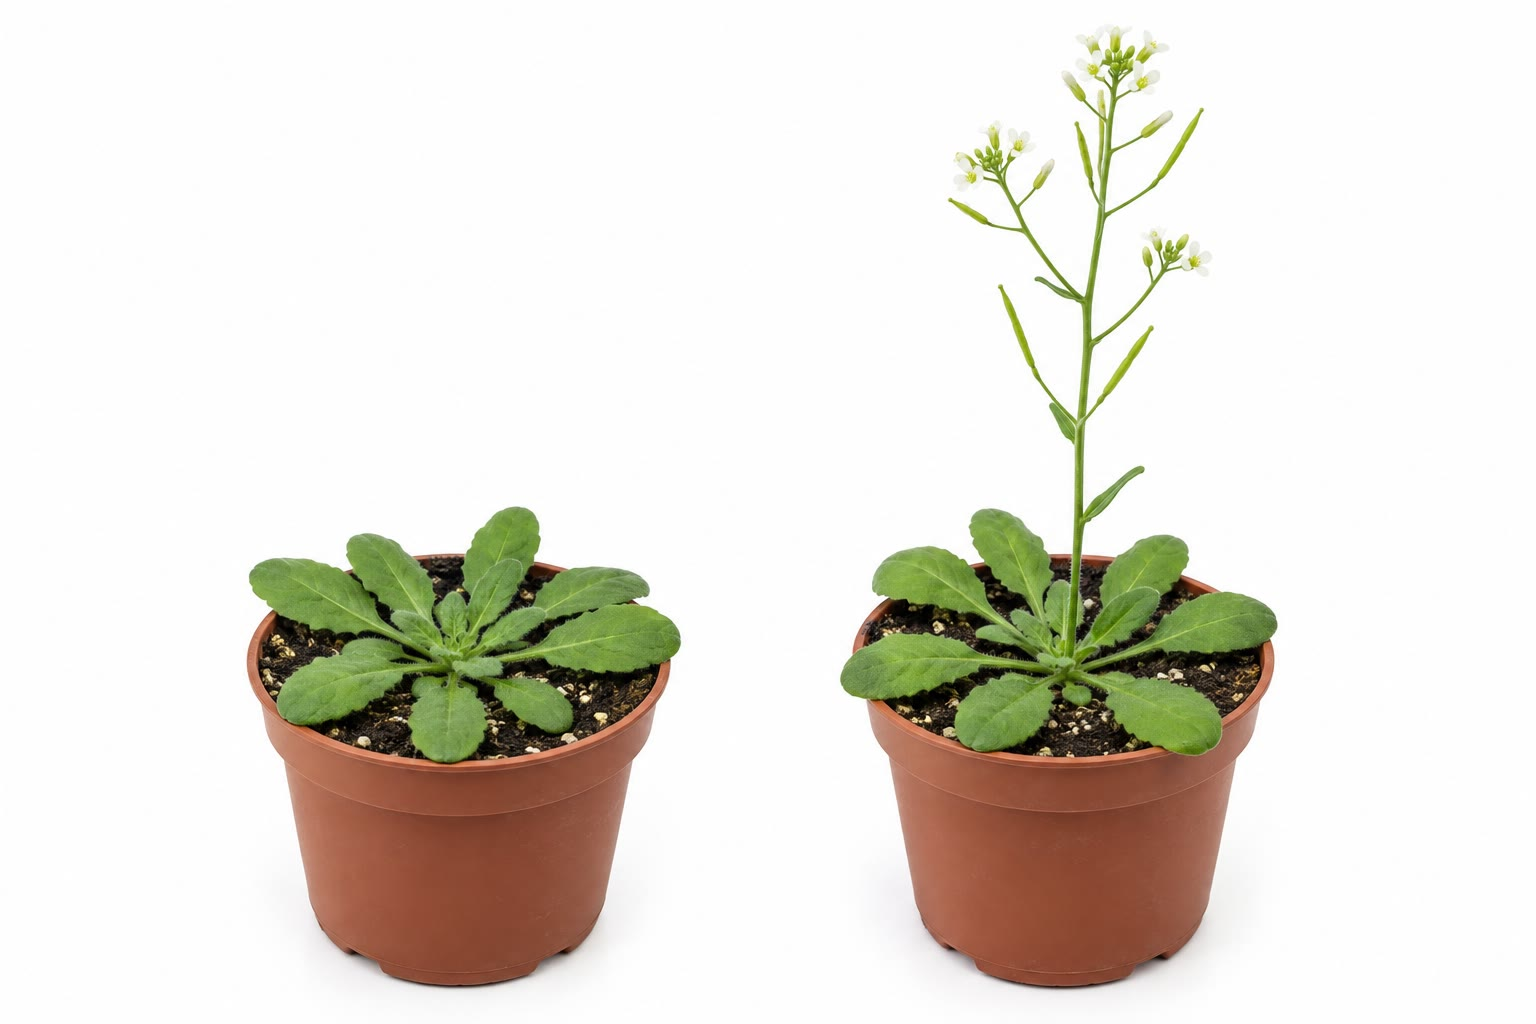
\includegraphics[width=0.58\linewidth]{images/book4/ai/b4-14-arabidopsis-daylength.jpg}

{\small \emph{Arabidopsis}, यानी कोई \omterm{prop:b2:plant-flowering:photoperiod}{दीर्घदिवसी पौधा}: छोटे दिनों में
पत्तियों का एक चक्रक; और लंबे दिनों में ले जाने पर वह सप्ताहों में
तना खींचकर फूल जाता है।}
\end{omfigure}

\begin{proposition}[वसंतीकरण: पौधा ठंड गिनता है]\label{prop:b2:plant-flowering:vernalisation}
\index{वसंतीकरण}\index{FLOWERING LOCUS C}
शीतकालीन अनाज, द्विवर्षी (गाजर, पत्तागोभी, फ़ॉक्सग्लव) और ठंडी जलवायु के
अनेक बहुवर्षी तब तक नहीं फूलते जब तक उन्होंने सप्ताहों की ठंड न झेल ली हो
--- यानी \emph{वसंतीकरण} --- जो यह सुनिश्चित करता है कि शरद में
अंकुरित होता कोई पौधा पाले में फूलने के बजाय वसंत की प्रतीक्षा करे।
उस ठंड को \omterm{def:b2:plant-meristems:meristem}{विभज्योतक} स्वयं भाँपता है, पत्तियाँ नहीं; उसे किसी दूसरे
उपचार से बदला नहीं जा सकता; और उसका प्रभाव उस पौधे की बाक़ी वृद्धि भर,
सैकड़ों कोशिका-विभाजनों के आरपार, याद रखा जाता है, पर
\omterm{def:b2:meiosis-heredity:meiosis}{अर्धसूत्री विभाजन} के आरपार नहीं --- हर \omterm{def:b2:angiosperm-reproduction:seed}{बीज} अवसंतीकृत ही आरंभ होता है।
\emph{Arabidopsis} में वह स्मृति एक जीन है, \emph{\omterm{prop:b2:plant-flowering:vernalisation}{FLOWERING LOCUS C}}
(FLC), जिसका उत्पाद पुष्पन को दबाता है: सप्ताहों की ठंड उसके क्रोमैटिन
को दमनकारी चिह्नों से ढककर उसे उत्तरोत्तर चुप कर देती है, वह चुप्पी हर
विभाजन पर नक़ल होती है, और भ्रूण में मिटा दी जाती है। इस तरह वह पौधा
उस ठंड को काल पर \emph{समाकलित} करता है --- कुछ ठंडे दिन गिने नहीं जाते
--- और जिस उत्परिवर्ती में FLC न हो उसे कोई शीत ऋतु नहीं चाहिए।
\end{proposition}

\begin{theorem}[समाकलन किसी झूठे वसंत से क्यों बचाता है]\label{thm:b2:plant-flowering:integration}
मान लीजिए कोई दमनकारी ठंड के प्रति दिन अचर दर $\alpha$ से चुप किया जाता
है, इसलिए $n$ ठंडे दिनों के बाद अब भी सक्रिय अंश
$f_n = e^{-\alpha n}$ है, और पुष्पन तब अनुमत है जब $f < f_c$ हो।
आवश्यक ठंडे दिनों की संख्या $n_c = \ln(1/f_c)/\alpha$ है, और ---
चूँकि वह चुप्पी स्थिर है --- उन ठंडे दिनों का लगातार होना ज़रूरी नहीं:
गिनती उनके कुल की है। जिस पौधे का $n_c = 40$ दिन हो उसे न जनवरी का
पखवाड़े भर का पिघलाव धोखा देता है न अक्तूबर की कोई ठंडी लहर; जबकि जो पौधा
केवल वर्तमान ताप भाँपता वह पहले ही गर्म सप्ताह में फूल जाता। वही समाकलन,
किसी देहली के साथ, वह ढंग है जिससे वह पौधा प्रतिबद्ध होने से पहले संचित
दिन-लंबाई पढ़ता है; और दोनों ऐसे तंत्र के उदाहरण हैं जो किसी संकेत के
तात्क्षणिक मान के बजाय उसके \emph{समाकल} को उत्तर देता है।
\end{theorem}
\begin{proof}
यदि हर ठंडा दिन बची हुई सक्रिय प्रतियों का (या अब तक अचिह्नित
क्रोमैटिन का) कोई अंश $\alpha$ चुप करे, तो सक्रिय
अंश $f_{n+1} = (1 - \alpha)f_n \approx e^{-\alpha}f_n$ का पालन करता है,
इसलिए $f_n = e^{-\alpha n}$, जिसमें $n$ ठंडे दिनों की गिनती है; और
असमिका $e^{-\alpha n} < f_c$ $n > \ln(1/f_c)/\alpha$ देती है।
जो दिन ठंडे नहीं वे न जोड़ते हैं न घटाते, क्योंकि वे चिह्न
स्थिर हैं, इसलिए केवल कुल ही मायने रखता है।
\end{proof}

\section{पुष्प का निर्माण: ABC मॉडल}

\begin{proposition}[ABC मॉडल]\label{prop:b2:plant-flowering:abc}
\index{ABC मॉडल}\index{समरूपांतरी जीन!पुष्पीय}
कोई पुष्पीय \omterm{def:b2:plant-meristems:meristem}{विभज्योतक} चार संकेंद्री चक्र बिछाता है: बाह्यदल, दलपत्र,
\omterm{def:b2:angiosperm-reproduction:flower}{पुंकेसर}, \omterm{def:b2:angiosperm-reproduction:flower}{अंडप}। उनकी पहचान \emph{समरूपांतरी जीनों} के तीन वर्ग तय करते
हैं, जो अतिव्यापी वलयों में काम करते हैं: चक्र 1 में अकेला वर्ग A
बाह्यदल देता है; चक्र 2 में A और B मिलकर दलपत्र देते हैं;
चक्र 3 में B और C मिलकर \omterm{def:b2:angiosperm-reproduction:flower}{पुंकेसर} देते हैं; और चक्र 4 में अकेला C
\omterm{def:b2:angiosperm-reproduction:flower}{अंडप} देता है। A और C एक-दूसरे को दबाते हैं, इसलिए जहाँ एक खो जाए वहाँ
दूसरा पूरे \omterm{def:b2:angiosperm-reproduction:flower}{पुष्प} पर फैल जाता है। ये नियम हर एकल
उत्परिवर्ती की भविष्यवाणी कर देते हैं: B खोइए और वह \omterm{def:b2:angiosperm-reproduction:flower}{पुष्प}
बाह्यदल--बाह्यदल--अंडप--अंडप हो जाता है;
C खोइए और वह बाह्यदल--दलपत्र--दलपत्र--बाह्यदल हो जाता है, और फिर भीतर एक
और \omterm{def:b2:angiosperm-reproduction:flower}{पुष्प}, क्योंकि C \omterm{def:b2:plant-meristems:meristem}{विभज्योतक} को रोकता भी है; और A खोइए तो वह
अंडप--पुंकेसर--पुंकेसर--अंडप हो जाता है। इनमें से अधिकांश जीन एक ही कुल
(MADS-बॉक्स) के \omterm{prop:b2:cell-differentiation:transcriptional}{अनुलेखन कारक} कूटबद्ध करते हैं, और तीनों कार्यों के लिए
एक चौथा वर्ग, E, चाहिए; और किसी पत्ती में B तथा C को एक साथ अभिव्यक्त
करने पर वह \omterm{def:b2:angiosperm-reproduction:flower}{पुंकेसर} जैसा अंग बन जाती है। बग़ीचों के
दोहरे \omterm{def:b2:angiosperm-reproduction:flower}{पुष्प} --- गुलाब, चपरासी, कमीलिया --- वर्ग-C
उत्परिवर्ती हैं, जिनके \omterm{def:b2:angiosperm-reproduction:flower}{पुंकेसर} अतिरिक्त दलपत्रों में बदल गए हैं।
\end{proposition}
\begin{proof}[प्रमाण-सामग्री]
कोएन और मेयरोविट्ज़ (1991) ने \emph{Arabidopsis} के और स्नैपड्रैगन के
समरूपांतरी उत्परिवर्तियों की तुलना की: दोनों में तीन वर्गों के
\omterm{def:b2:genome-diversification:mutation}{उत्परिवर्तन} हर बार दो आसन्न चक्र बदल देते थे, और वही जोड़ियाँ,
और उत्परिवर्तियों के संयोजन वैसे ही बरते जैसे वह मॉडल कहता है (उनका
त्रिगुण उत्परिवर्ती केवल पत्तियाँ बनाता है)। क्लोनन ने दिखाया कि वे जीन
भविष्यवाणी किए गए वलयों में अभिव्यक्त होने वाले \omterm{prop:b2:cell-differentiation:transcriptional}{अनुलेखन कारक} हैं; और किसी
B जीन को चारों चक्रों में सक्रिय किसी उन्नायक के नीचे रखने पर
दलपत्र--दलपत्र--पुंकेसर--पुंकेसर मिला।
\end{proof}

\begin{omfigure}
\begin{tikzpicture}[every node/.style={font=\scriptsize}]
  % four whorls as columns
  \foreach \x/\w in {0/{चक्र 1}, 2.2/{चक्र 2}, 4.4/{चक्र 3}, 6.6/{चक्र 4}} \node[above] at (\x+0.9,3.3) {\w};
  \fill[omDef!35] (0,2.4) rectangle (4.2,3.1); \node at (2.1,2.75) {A};
  \fill[omProp!40] (2.2,1.6) rectangle (6.4,2.3); \node at (4.3,1.95) {B};
  \fill[omThm!30] (4.4,0.8) rectangle (8.6,1.5); \node at (6.5,1.15) {C};
  \foreach \x/\o in {0/{बाह्यदल}, 2.2/{दलपत्र}, 4.4/{पुंकेसर}, 6.6/{अंडप}} \node[below, align=center] at (\x+0.9,0.6) {\o};
  \node[anchor=west, align=left] at (9.2,3.0) {वन्य प्ररूप: A, AB, BC, C};
  \node[anchor=west, align=left] at (9.2,2.3) {B नहीं: बाह्यदल, बाह्यदल, अंडप, अंडप};
  \node[anchor=west, align=left] at (9.2,1.6) {C नहीं: बाह्यदल, दलपत्र, दलपत्र, बाह्यदल\ldots};
  \node[anchor=west, align=left] at (9.2,0.9) {A नहीं: अंडप, पुंकेसर, पुंकेसर, अंडप};
\end{tikzpicture}

{\small \omterm{prop:b2:plant-flowering:abc}{ABC मॉडल}। अतिव्यापी वलयों में तीन जीन-वर्ग
चारों अंग-पहचान तय करते हैं; किसी एक वर्ग के खोने से दो चक्र बदल जाते
हैं, और वे उत्परिवर्ती \omterm{def:b2:angiosperm-reproduction:flower}{पुष्प} ठीक वही हैं जिनकी भविष्यवाणी की गई थी।}
\end{omfigure}

\begin{omfigure}
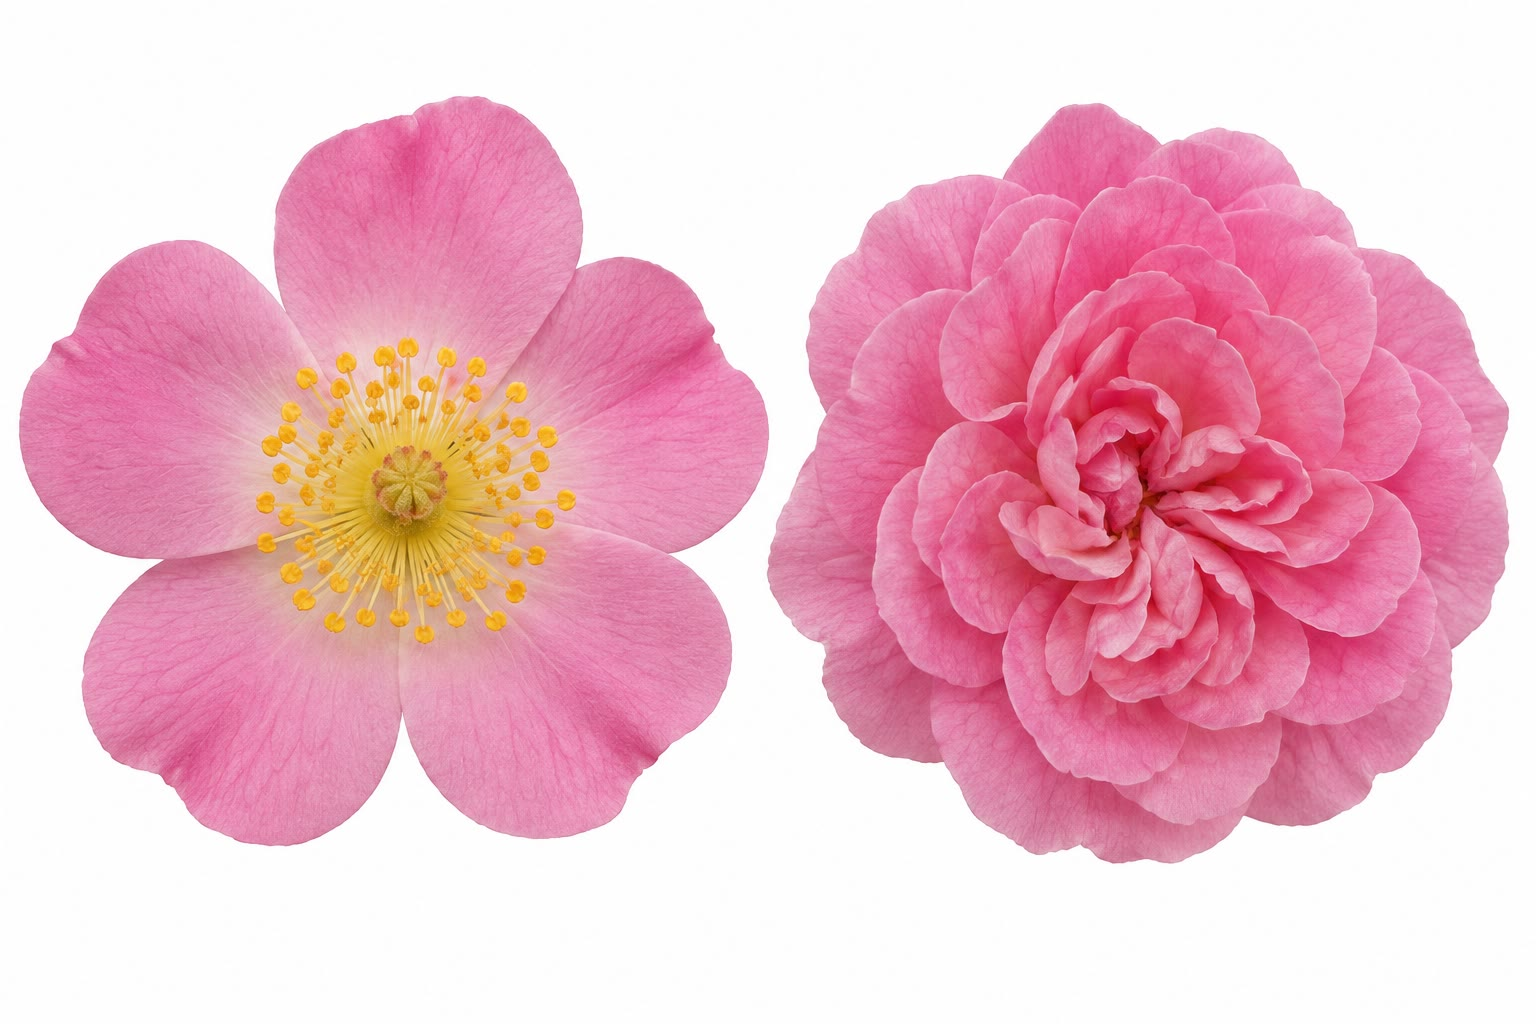
\includegraphics[width=0.58\linewidth]{images/book4/ai/b4-14-double-flower.jpg}

{\small किसी वन्य-प्ररूप \omterm{def:b2:angiosperm-reproduction:flower}{पुष्प} के बग़ल एक दोहरा रूप: उसके \omterm{def:b2:angiosperm-reproduction:flower}{पुंकेसर}
दलपत्र बन चुके हैं --- यानी कोई वर्ग-C उत्परिवर्ती, जिसे मालियों ने
सदियों तक चुना, किसी के यह जाने से पहले कि वह दोहरा क्यों है।}
\end{omfigure}

\section{प्रसुप्ति और अंकुरण}

\begin{definition}[बीज प्रसुप्ति]\label{def:b2:plant-flowering:dormancy}
\index{प्रसुप्ति!बीज}\index{ऐब्सिसिक अम्ल}\index{जिबरेलिन}\index{स्तरीकरण}
जो जीवनक्षम \omterm{def:b2:angiosperm-reproduction:seed}{बीज} ऐसी परिस्थितियों में अंकुरित न हो जो वृद्धि सँभाल
सकती हों वह \emph{प्रसुप्त} है। \omterm{def:b2:angiosperm-reproduction:seed}{प्रसुप्ति} \omterm{def:b2:angiosperm-reproduction:seed}{बीज} के
परिपक्वन में \emph{ऐब्सिसिक अम्ल} (ABA) थोपता है, जो भंडारों का
संचय और भ्रूण का सूखना भी चलाता है, और उसे
\omterm{def:b2:angiosperm-reproduction:seed}{बीज-आवरण} बनाए रखता है (जो जल या ऑक्सीजन के लिए अपारगम्य होता है, या
यांत्रिक रूप से रोकता है) या स्वयं भ्रूण की अवस्था। वह
उन्हीं संकेतों से टूटती है जो प्रतिकूल ऋतु का अंत बताते हैं:
सप्ताहों की ठंड और नमी (\emph{स्तरीकरण}, यानी \omterm{def:b2:angiosperm-reproduction:seed}{बीज} का
वसंतीकरण), प्रकाश --- उन छोटे \omterm{def:b2:angiosperm-reproduction:seed}{बीजों} के लिए जिन्हें सतह के पास होना
चाहिए, और जिसे फ़ाइटोक्रोम भाँपता है --- या अंधकार, बदलते
ताप, वर्षा से संदमकों का बह जाना, मिट्टी या किसी आँत से उस
आवरण का खुरचा जाना, और आग के बाद धुआँ तथा ताप। वह
निर्णय ABA और \emph{जिबरेलिन} के बीच का संतुलन है: तोड़ने वाले संकेत ABA
गिराते और जिबरेलिन चढ़ाते हैं, जो उन भंडारों को गतिशील करती है
(\cref{ch:b2:angiosperm-reproduction}) और मूलांकुर को बढ़ने देती है।
\omterm{def:b2:angiosperm-reproduction:seed}{बीजों} की कोई आबादी एकरूप नहीं होती: एक अंश
पहले ही अवसर पर अंकुरित होता है, और बाक़ी वर्ष भर या अधिक प्रतीक्षा करते
हैं, ताकि कोई एक बुरी ऋतु पूरे दल को न मार डाले --- यानी
\emph{\omterm{def:b2:angiosperm-reproduction:seed}{बीज} बैंक}, किसी अप्रत्याशित संसार के विरुद्ध एक बचाव।
\end{definition}
\begin{proof}[प्रमाण-सामग्री]
सलाद के \omterm{def:b2:angiosperm-reproduction:seed}{बीज} (बोर्थविक, 1952) अँधेरे में लाल प्रकाश की एक झलक के
बाद अंकुरित होते हैं और दूर-लाल की झलक के बाद नहीं; और लाल, फिर
दूर-लाल, फिर लाल दिए जाएँ तो वे अंकुरित होते हैं --- यानी अंतिम झलक ही
निर्णय करती है। वही प्रतिवर्ती रंजक, जो पुष्पन का समय तय करता है, अंकुरण
आरंभ करता है। अनेक वृक्षों के \omterm{def:b2:angiosperm-reproduction:seed}{बीज} ताज़े ही गर्म मिट्टी में बोए जाएँ तो
कुछ नहीं करते; जबकि वही
\omterm{def:b2:angiosperm-reproduction:seed}{बीज} किसी नम प्रशीतक में दो महीने रहने के बाद तुरंत अंकुरित होते हैं,
और ABA-न्यून उत्परिवर्ती \omterm{def:b2:angiosperm-reproduction:seed}{बीज} के सूखने से भी पहले पौधे पर ही अंकुरित हो
जाते हैं।
\end{proof}

\begin{omfigure}
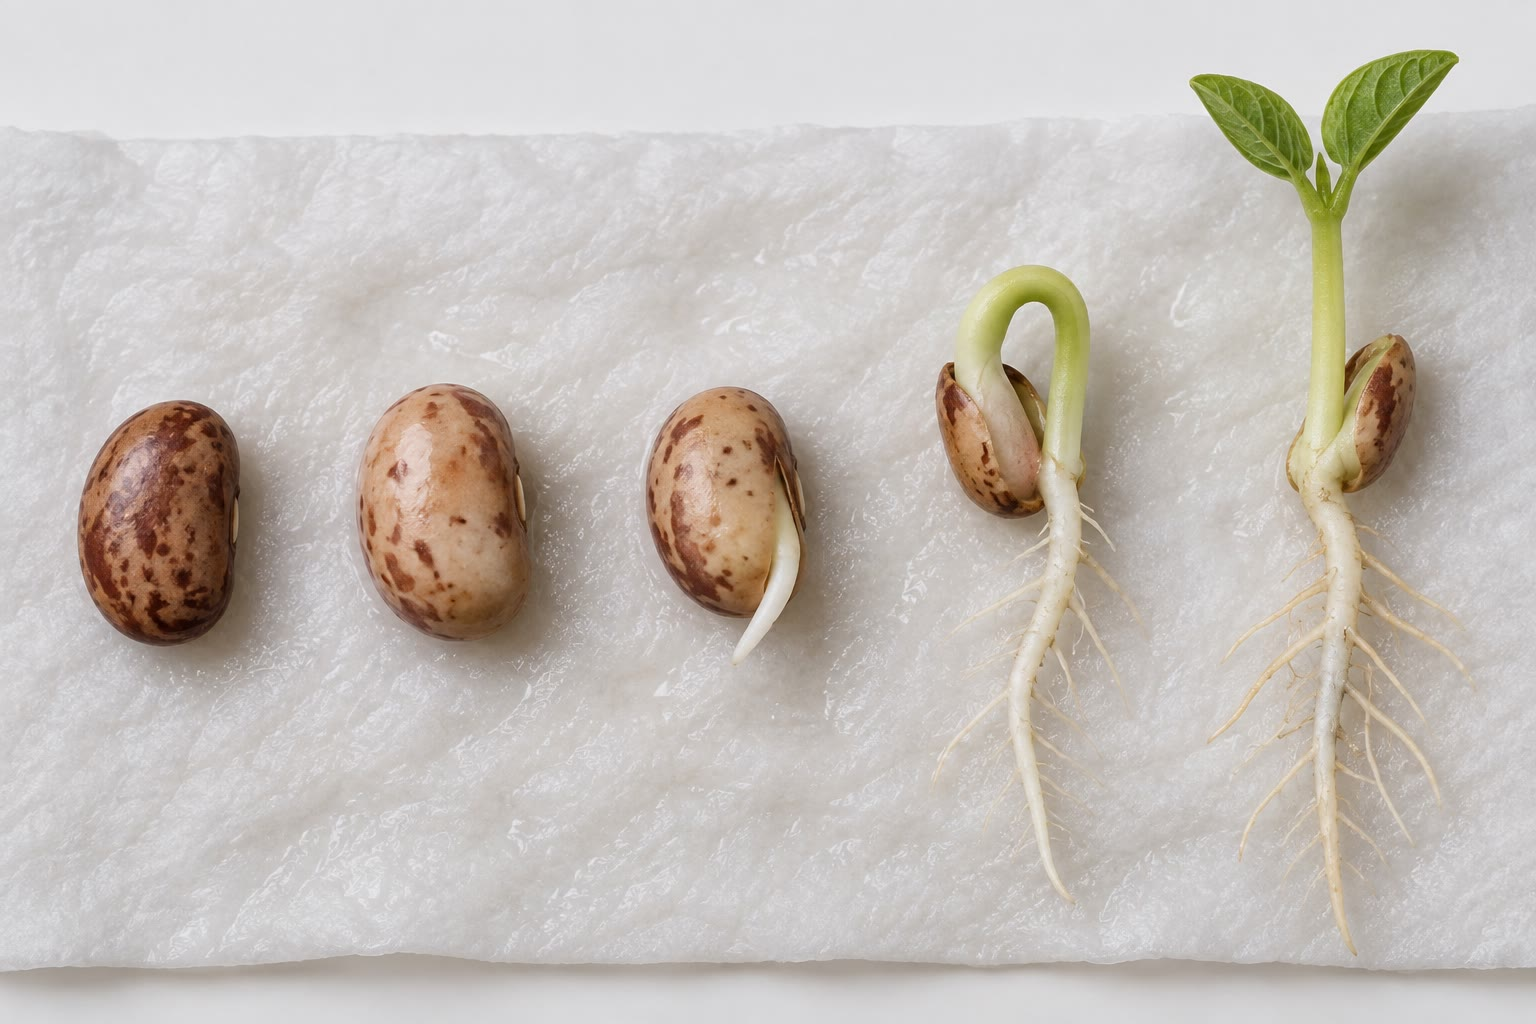
\includegraphics[width=0.66\linewidth]{images/book4/ai/b4-14-germinating-beans.jpg}

{\small सेम का अंकुरण: वह \omterm{def:b2:angiosperm-reproduction:seed}{बीज} जल सोखता है, मूलांकुर पहले निकलता है,
बीजपत्रोपरिक अक्ष मिट्टी में से अंकुड़े की तरह ऊपर उठता है, और प्रकाश में
वह अंकुड़ा सीधा हो जाता है तथा पहली पत्तियाँ खुल जाती हैं।}
\end{omfigure}

\begin{theorem}[अंकुरण एक दाँव के रूप में]\label{thm:b2:plant-flowering:bet}
\index{दाँव-बँटाई}
मान लीजिए किसी बीज-दल का एक अंश $g$ हर वर्ष अंकुरित होता है और
बाक़ी $s$ प्रायिकता से मिट्टी में अगले वर्ष तक बचा रहता है।
किसी अच्छे वर्ष में कोई अंकुरित होता \omterm{def:b2:angiosperm-reproduction:seed}{बीज} $R_g$ \omterm{def:b2:angiosperm-reproduction:seed}{बीज} छोड़ता है; किसी बुरे
वर्ष में कोई नहीं; और वर्ष $p$ प्रायिकता से अच्छे होते हैं। जो रणनीति
सब कुछ एक साथ अंकुरित कर दे ($g = 1$) उसकी, वर्षों की किसी दौड़ पर,
दीर्घकालिक वृद्धि दर $\ln$-औसत के रूप में $p\ln R_g + (1 - p)\ln 0 =
-\infty$ है: यानी एक ही बुरा वर्ष उसे मिटा देता है। जिस रणनीति में
$g < 1$ हो वह अच्छे वर्षों में $gR_g + (1 - g)s$ गुणक से और बुरे वर्षों
में $(1 - g)s > 0$ गुणक से बढ़ती है, इसलिए उसकी दीर्घकालिक दर,
\[
r = p\ln\bigl(gR_g + (1 - g)s\bigr) + (1 - p)\ln\bigl((1 - g)s\bigr),
\]
परिमित है और, $p$ के 1 के बहुत पास न होने पर, किसी मध्यवर्ती $g$ पर
अधिकतम होती है। $R_g = 20$, $s = 0.8$ और $p = 0.7$ के साथ
उसका इष्टतम $g = 0.7$ के पास है: यानी अधिकांश अंकुरित कीजिए, कुछ बचाकर रखिए।
\omterm{def:b2:angiosperm-reproduction:seed}{प्रसुप्ति} अंकुरित होने में विफलता नहीं बल्कि एक विकसित आंशिक
इनकार है।
\end{theorem}
\begin{proof}
$T$ वर्षों बाद आबादी का आकार वार्षिक गुणकों का गुणनफल है,
इसलिए उसकी वृद्धि दर उनके लघुगणकों का औसत है
(यानी गुणोत्तर माध्य दर), और लंबी दौड़ों पर वरण इसी को अधिकतम करता है।
$g = 1$ के साथ बुरे वर्ष का गुणक शून्य है और उसका लघुगणक
$-\infty$। $g < 1$ के लिए दोनों गुणक धनात्मक हैं; और $r$ का $g$ के
सापेक्ष अवकलन करके उसे शून्य रखने पर वह इष्टतम मिलता है, जो उद्धृत
आँकड़ों के लिए $g = 0.7$ के पास पड़ता है
($r$ को $g = 0.4, 0.6, 0.8, 1$ पर निकालने से $1.28$, $1.42$,
$1.40$, $-\infty$ मिलते हैं)।
\end{proof}

\begin{omfigure}
\begin{tikzpicture}
\begin{axis}[
  width=0.7\linewidth, height=5.4cm,
  axis x line=bottom, axis y line=left,
  xmin=0, xmax=1, ymin=0, ymax=1.7,
  xlabel={हर वर्ष अंकुरित होता अंश, $g$}, ylabel={दीर्घकालिक वृद्धि दर $r$},
  xlabel style={font=\small, at={(axis description cs:0.5,-0.13)}, anchor=north},
  ylabel style={font=\small},
  tick label style={font=\small}, xtick={0,0.2,0.4,0.6,0.8,1}, ytick={0,0.5,1,1.5},
  clip=false,
]
\addplot[very thick, omDef, domain=0.02:0.97, samples=100] {0.7*ln(20*x + 0.8*(1-x)) + 0.3*ln(0.8*(1-x))};
\draw[dashed, gray] (axis cs:0.7,0) -- (axis cs:0.7,1.43);
\node[font=\scriptsize, anchor=south] at (axis cs:0.7,1.45) {इष्टतम: \qty{30}{\%} मिट्टी में रखिए};
\node[font=\scriptsize, anchor=north west, align=left] at (axis cs:0.7,0.6) {$g \to 1$: एक बुरा वर्ष\\उस दल को मिटा देता है};
\end{axis}
\end{tikzpicture}

{\small \omterm{def:b2:angiosperm-reproduction:seed}{प्रसुप्ति} से \omterm{thm:b2:plant-flowering:bet}{दाँव-बँटाई}। दस में सात वर्ष अच्छे हों तो
जो दल पूरा का पूरा अंकुरित हो जाए वह अंततः किसी बुरे वर्ष से नष्ट हो
जाता है; जबकि जो दल अपने \omterm{def:b2:angiosperm-reproduction:seed}{बीजों} का एक हिस्सा रोक रखे वह लंबी दौड़ में
सबसे तेज़ बढ़ता है।}
\end{omfigure}

\section{अभ्यास}

\begin{exercise}[$\star$]\label{exo:b2:plant-flowering:1}
कायिक, पुष्पक्रम और पुष्पीय \omterm{def:b2:plant-meristems:meristem}{विभज्योतकों} में भेद कीजिए, और
बताइए कि कौन-से निश्चित हैं।
\end{exercise}

\begin{exercise}[$\star$]\label{exo:b2:plant-flowering:2}
अल्पदिवसी, दीर्घदिवसी और दिन-उदासीन पौधों की परिभाषा हर एक के एक
उदाहरण सहित दीजिए, और बताइए कि कोई \omterm{prop:b2:plant-flowering:photoperiod}{अल्पदिवसी पौधा} असल में क्या नापता है।
\end{exercise}

\begin{exercise}[$\star$]\label{exo:b2:plant-flowering:3}
वन्य प्ररूप में और \omterm{prop:b2:plant-flowering:abc}{ABC मॉडल} के तीनों एकल उत्परिवर्तियों में हर चक्र
की अंग-पहचान बताइए।
\end{exercise}

\begin{exercise}[$\star$]\label{exo:b2:plant-flowering:4}
बीज-प्रसुप्ति तोड़ने वाले चार संकेत बताइए और हर एक के लिए वह ऋतु
या स्थान जो वह बताता है।
\end{exercise}

\begin{exercise}[$\star\star$]\label{exo:b2:plant-flowering:5}
किसी अल्पदिवसी पौधे की क्रांतिक रात \qty{10}{h} है। बताइए कि वह इनमें
फूलता है या नहीं: \qty{16}{h} प्रकाश/\qty{8}{h} अंधकार; \qty{12}{h}/\qty{12}{h};
\qty{12}{h} प्रकाश, \qty{6}{h} अंधकार, मिनट भर प्रकाश, \qty{6}{h} अंधकार;
\qty{8}{h} प्रकाश, \qty{4}{h} अंधकार, \qty{4}{h} प्रकाश, \qty{8}{h} अंधकार।
\end{exercise}

\begin{exercise}[$\star\star$]\label{exo:b2:plant-flowering:6}
किसी प्रेरित अल्पदिवसी पौधे की एक पत्ती लंबे दिनों में रखे किसी
दीर्घदिवसी पौधे पर ग्राफ़्ट की जाती है, और वह \omterm{prop:b2:plant-flowering:photoperiod}{दीर्घदिवसी पौधा} फूल जाता
है। यह \omterm{def:b2:plant-flowering:florigen}{फ़्लोरिजन} के बारे में क्या दिखाता है? और यदि वह ग्राफ़्ट ऐसी
पत्ती से किया जाए जो प्रेरित तो है पर जिसका फ्लोएम वृंत पर काट दिया गया
हो, तो?
\end{exercise}

\begin{exercise}[$\star\star$]\label{exo:b2:plant-flowering:7}
ठंड उस दमनकारी को प्रति दिन $\alpha = 0.05$ से चुप करती है और
पुष्पन को $f < 0.15$ चाहिए। कितने ठंडे दिन चाहिए? किसी
शीत ऋतु में 15, 12 और 20 दिनों की तीन ठंडी लहरें हैं जिनके बीच
पिघलाव हैं: क्या वह पौधा वसंतीकृत है? और यदि $\alpha$ $0.02$ होता तो?
\end{exercise}

\begin{exercise}[$\star\star$]\label{exo:b2:plant-flowering:8}
समझाइए कि किसी वसंतीकृत पौधे की स्मृति उसके \omterm{def:b2:angiosperm-reproduction:seed}{बीजों} में क्यों खो जाती है,
क्रोमैटिन के पदों में, और यह उपयोगी क्यों है।
\end{exercise}

\begin{exercise}[$\star\star$]\label{exo:b2:plant-flowering:9}
सलाद के \omterm{def:b2:angiosperm-reproduction:seed}{बीजों} को अँधेरे में ये क्रम दिए जाते हैं: R; R फिर FR;
R, FR, R; R, FR, R, FR। हर स्थिति में अंकुरण की भविष्यवाणी कीजिए और
फ़ाइटोक्रोम के दोनों रूपों के पदों में समझाइए।
\end{exercise}

\begin{exercise}[$\star\star\star$]\label{exo:b2:plant-flowering:10}
\omterm{thm:b2:plant-flowering:bet}{दाँव-बँटाई} मॉडल में $R_g = 20$, $s = 0.8$ के साथ,
$g = 0.4$, $0.6$, $0.8$ और $1$ के लिए दीर्घकालिक वृद्धि दर तब निकालिए
जब $p = 0.7$ हो, और फिर $p = 0.95$ पर भी। इष्टतम कैसे खिसकता है,
और यह रेगिस्तानों बनाम घास-मैदानों के लिए क्या भविष्यवाणी करता है?
\end{exercise}

\begin{exercise}[$\star\star\star$]\label{exo:b2:plant-flowering:11}
इनसे बनने वाले \omterm{def:b2:angiosperm-reproduction:flower}{पुष्प} की भविष्यवाणी कीजिए: किसी वर्ग-B जीन को चारों
चक्रों में अभिव्यक्त करना; वर्ग C को चारों में अभिव्यक्त करना; और A तथा B
से रहित कोई दोहरा उत्परिवर्ती। फिर समझाइए कि C-रहित \omterm{def:b2:angiosperm-reproduction:flower}{पुष्प}
चक्र बनाता क्यों चला जाता है।
\end{exercise}

\begin{exercise}[$\star\star\star$]\label{exo:b2:plant-flowering:12}
``कोई पौधा उन संकेतों को समाकलित करके फूलने का निर्णय करता है जिन पर उसका
कोई वश नहीं।'' इस अध्याय के तीनों समाकलनों पर --- दिन-लंबाई का, ठंड का,
और \omterm{def:b2:angiosperm-reproduction:seed}{बीज} बैंक के वर्षों का --- और इस पर विचार कीजिए कि कोई समाकलक उस पौधे
को किससे बचाता है जिससे कोई सरल देहली नहीं बचाती।
\end{exercise}

\section{समस्या: उगाने वाले का पंचांग}

\begin{problem}[{सप्तांत समस्या --- गुलदाउदी उगाने वाला बत्तियों से
पुष्पन की सारणी बिठाता है, कोई गेहूँ-प्रजनक ठंड गिनता है, किसी फूलवाले
का दोहरा पुष्प समझाया जाता है, और किसी बीज-लॉट की प्रसुप्ति का प्रतिरूप
बनाया जाता है, और अंत उस रात्रि-लंबाई पर जो उस फ़सल को चलाती है, उन ठंडे
दिनों पर जो उस गेहूँ को चाहिए, और सर्वोत्तम अंकुरण-अंश पर}]
\label{pb:b2:plant-flowering:1}
गुलदाउदी \omterm{prop:b2:plant-flowering:photoperiod}{अल्पदिवसी पौधा} है जिसकी क्रांतिक रात्रि-लंबाई
\qty{9.5}{h} है; प्रेरण के लिए \num{12} लगातार प्रेरक
रातें चाहिए, और \omterm{def:b2:angiosperm-reproduction:flower}{पुष्प} प्रेरण के \num{8} सप्ताह बाद खुलते हैं। नवंबर में
वह हरितगृह 17:00 से 07:30 तक अँधेरा रहता है। शीत-गेहूँ
का प्रति ठंडा दिन $\alpha = 0.06$ है और वह तब फूलता है जब $f < 0.10$ हो। \omterm{def:b2:angiosperm-reproduction:seed}{बीज}
लॉट: $R_g = 15$, $s = 0.7$, और वर्ष $p$ प्रायिकता से अच्छे।

\medskip
\noindent\textbf{भाग I --- हरितगृह।}
\begin{enumerate}
  \item जून में प्राकृतिक रात \qty{8}{h} की है। क्या वह फ़सल
        फूलेगी? अगस्त में \omterm{def:b2:angiosperm-reproduction:flower}{पुष्प} बेचने के लिए उगाने वाले को क्या करना पड़ेगा?
  \item वह उगाने वाला उस फ़सल को 19:00 से 07:00 तक काले कपड़े से
        ढकता है। वह पौधा कौन-सी रात्रि-लंबाई देखता है, और
        15~अगस्त को खिलने के लिए ढकना कब आरंभ होना चाहिए?
  \item नवंबर में प्राकृतिक रात \qty{14}{h} की है और वह उगाने वाला
        पुष्पन को क्रिसमस तक \emph{टालना} चाहता है। कोई प्रकाश-सारणी
        सुझाइए और समझाइए कि एक छोटी झलक क्यों पर्याप्त है।
  \item वह झलक 00:00 के बजाय 21:00 पर दी जाती है,
        और प्रेरण रुकता नहीं। क्रांतिक रात्रि-लंबाई से समझाइए।
  \item उन बारह में से एक रात वह कपड़ा डालना छूट जाता है। भविष्यवाणी
        कीजिए, और बताइए कि कोई कॉकलबर क्या करता।
  \item वह झलक हरे प्रकाश में दी जाए तो विफल होती है; लाल प्रकाश में
        चलती है; और लाल के बाद दूर-लाल हो तो विफल। समझाइए।
  \item किसी प्रेरित पौधे की एक पत्ती लंबे दिनों में रखे किसी पौधे पर
        ग्राफ़्ट की जाती है। भविष्यवाणी कीजिए, और बताइए कि यह किसकी पहचान कराता है।
\end{enumerate}

\medskip
\noindent\textbf{भाग II --- गेहूँ।}
\begin{enumerate}[resume]
  \item उस गेहूँ को कितने ठंडे दिन चाहिए?
  \item अक्तूबर में बोए जाने पर उसे नवंबर में 10 ठंडे दिन मिलते हैं,
        दिसंबर हलका रहता है, जनवरी में 25 और फ़रवरी में 12। वह कब
        वसंतीकृत होता है?
  \item मार्च में बोए जाने पर उसे 6 ठंडे दिन मिलते हैं। क्या वह उस
        ग्रीष्म फूलता है? कृषि पर इसका क्या परिणाम है?
  \item किसी उत्परिवर्ती में वह दमनकारी नहीं है। उसके व्यवहार की
        भविष्यवाणी कीजिए और बताइए कि प्रजनक ऐसे गेहूँ को ``वसंत गेहूँ'' क्यों कहते हैं।
  \item समझाइए कि ठंड की स्मृति वसंत भर \omterm{def:b2:plant-meristems:meristem}{विभज्योतक} के विभाजनों को क्यों
        झेल जाती है पर अगली पीढ़ी बनाने वाले \omterm{def:b2:meiosis-heredity:meiosis}{अर्धसूत्री विभाजन} को क्यों
        नहीं।
  \item दिन-लंबाई के विपरीत, ठंड \omterm{def:b2:plant-meristems:meristem}{विभज्योतक} में ही क्यों गिनी जानी
        चाहिए, पत्तियों में क्यों नहीं?
\end{enumerate}

\medskip
\noindent\textbf{भाग III --- फूलवाला।}
\begin{enumerate}[resume]
  \item किसी दोहरे गुलाब में वहाँ दलपत्र हैं जहाँ \omterm{def:b2:angiosperm-reproduction:flower}{पुंकेसर} होने चाहिए,
        और बीच में कुछ अतिरिक्त दलपत्र भी। किस वर्ग का जीन विफल हुआ
        है? चक्र-सूत्र दीजिए।
  \item ऐसे गुलाब पराग-जनक के रूप में बंध्य होते हैं पर कभी-कभी
        \omterm{def:b2:angiosperm-reproduction:seed}{बीज} बाँध लेते हैं। \omterm{prop:b2:plant-flowering:abc}{ABC मॉडल} से दोनों तथ्य समझाइए।
  \item किसी स्नैपड्रैगन में दलपत्रों की जगह \omterm{def:b2:angiosperm-reproduction:flower}{पुंकेसर} और बाह्यदलों की
        जगह \omterm{def:b2:angiosperm-reproduction:flower}{अंडप} हैं। कौन-सा वर्ग विफल हुआ है?
  \item ऐसे पौधे के \omterm{def:b2:angiosperm-reproduction:flower}{पुष्प} की भविष्यवाणी कीजिए जिसमें वर्ग C अपने
        सामान्य चक्रों के साथ-साथ चक्र 1 में भी अभिव्यक्त हो।
  \item उन्हीं \omterm{def:b2:genome-diversification:mutation}{उत्परिवर्तनों} ने किसी गुलाब, किसी स्नैपड्रैगन और
        \emph{Arabidopsis} में, जो दस करोड़ वर्ष से अलग हैं, वही
        रूपांतर क्यों बनाए?
  \item किसी वन्य-प्ररूप \omterm{def:b2:angiosperm-reproduction:flower}{पुष्प} के चक्र 2 में A और B दोनों सक्रिय हैं।
        यदि वहाँ केवल B सक्रिय होता तो उस अंग की भविष्यवाणी कीजिए।
\end{enumerate}

\medskip
\noindent\textbf{भाग IV --- \omterm{def:b2:angiosperm-reproduction:seed}{बीज} लॉट।}
\begin{enumerate}[resume]
  \item दीर्घकालिक वृद्धि दर $r$ को $g = 0.5$, $0.7$ और $0.9$ के लिए
        तब निकालिए जब $p = 0.8$ हो।
  \item इन तीनों में सबसे अच्छा कौन-सा है? $g = 1$ पर क्या होता है?
  \item $p = 0.5$ (किसी रेगिस्तान) के लिए फिर से निकालिए। अब कौन-सा
        $g$ सबसे अच्छा है?
  \item कोई उगाने वाला पूरा लॉट किसी अच्छे वर्ष में एक ही खेत में बोता
        है और प्रति \omterm{def:b2:angiosperm-reproduction:seed}{बीज} $R_g$ काटता है। समझाइए कि उसकी रणनीति उस पौधे
        की रणनीति से क्यों भिन्न है और किसी बुरे वर्ष के आरपार उस
        क़िस्म को बचाए रखने के लिए उसे क्या करना पड़ेगा।
  \item उन \omterm{def:b2:angiosperm-reproduction:seed}{बीजों} को अंकुरित होने के लिए प्रकाश चाहिए। किसी छोटे \omterm{def:b2:angiosperm-reproduction:seed}{बीज} के
        लिए इसका अनुकूली अर्थ समझाइए, और भविष्यवाणी कीजिए कि जुताई
        उस \omterm{def:b2:angiosperm-reproduction:seed}{बीज} बैंक का क्या करती है।
  \item परिणाम बताइए: क्रांतिक रात्रि-लंबाई और ढकने की
        सारणी, गेहूँ की ठंड-माँग, और सर्वोत्तम $g$, $p = 0.8$ तथा
        $p = 0.5$ के लिए।
\end{enumerate}
\end{problem}
